\documentclass{article}
\usepackage[T1]{fontenc}
\usepackage{amssymb, amsmath, graphicx, subfigure, enumerate}
\usepackage{amsthm,alltt} 
\usepackage[margin=1.25in]{geometry} %geometry (sets margin) and other useful packages
\usepackage{tikz}
\usepackage{graphicx,ctable,booktabs}
\usepackage{mathtools}
\usepackage[boxed]{algorithm2e}
\usepackage{mathdots}
\usepackage{fancyhdr} %Fancy-header package to modify header/page numbering
\usepackage{cleveref}

\setlength{\oddsidemargin}{.25in}
\setlength{\evensidemargin}{.25in}
\setlength{\textwidth}{6in}
\setlength{\topmargin}{-0.4in}
\setlength{\textheight}{8.5in}



\newcommand{\heading}[6]{
  \renewcommand{\thepage}{\arabic{page}} % used to be #1-\arabic{page}
  \noindent
  \begin{center}
  \framebox{
    \vbox{
      \hbox to 5.78in { \textbf{#2} \hfill #3 }
      \vspace{4mm}
      \hbox to 5.78in { {\Large \hfill #6  \hfill} }
      \vspace{2mm}
      \hbox to 5.78in { \textit{Instructor: #4 \hfill #5} }
    }
  }
  \end{center}
  \vspace*{4mm}
}

%Redefining sections as problems
\makeatletter
\newenvironment{problem}{\@startsection
       {section}
       {2}
       {-.2em}
       {-3.5ex plus -1ex minus -.2ex}
       {2.3ex plus .2ex}
       {\pagebreak[3]%forces pagebreak when space is small; use \eject for better results
       \large\bf\noindent{Problem }
       }
       }
       %{%\vspace{1ex}\begin{center} \rule{0.3\linewidth}{.3pt}\end{center}}
       %\begin{center}\large\bf \ldots\ldots\ldots\end{center}}
\makeatother


\newtheorem{theorem}{Theorem}[section]
\newtheorem{definition}[theorem]{Definition}
\newtheorem{remark}[theorem]{Remark}
\newtheorem{lemma}[theorem]{Lemma}
\newtheorem{corollary}[theorem]{Corollary}
\newtheorem{proposition}[theorem]{Proposition}
\newtheorem{claim}[theorem]{Claim}
\newtheorem{observation}[theorem]{Observation}
\newtheorem{fact}[theorem]{Fact}
\newtheorem{assumption}[theorem]{Assumption}

%\newenvironment{proof}{\noindent{\bf Proof:} \hspace*{1mm}}{
% \hspace*{\fill} $\Box$ }
%\newenvironment{proof_of}[1]{\noindent {\bf Proof of #1:}
% \hspace*{1mm}}{\hspace*{\fill} $\Box$ }
%\newenvironment{proof_claim}{\begin{quotation} \noindent}{
% \hspace*{\fill} $\diamond$ \end{quotation}}

\newcommand{\problemset}[3]{\heading{#1}{\classname}{#2}{\instructor}{#3}{Problem Set #1}} % Don't change this line
%%%%%%%%%%%%%%%%%%%%%%%%%% Change this stuff below, don't change the line above this one
\newcommand{\problemsetnum}{5}            % problem set number
\newcommand{\duedate}{2/26/2018} % problem set deadline
\newcommand{\studentname}{Student Name: }      % name of student (i.e., you)
\newcommand{\classname}{CS 8803 GA -- HW 5.  \ \ Due: \duedate \ \ \ Name:   }
%%%%%%%%%%%%%%%%%%%%%%%%%%

\pagestyle{fancy}
%\addtolength{\headwidth}{\marginparsep} %these change header-rule width
%\addtolength{\headwidth}{\marginparwidth}
\lhead{\classname} %Problem \thesection}
\chead{} 
\rhead{\thepage} 
%\lfoot{\small\scshape \classname}
\cfoot{} 
%\rfoot{\footnotesize PS \#\problemsetnum} 
\renewcommand{\headrulewidth}{.3pt} 
\renewcommand{\footrulewidth}{.3pt}
\setlength\voffset{-0.25in}
\setlength\textheight{648pt}


\newcommand{\sit}{\shortintertext}
\newcommand\deq{\mathrel{\overset{\makebox[0pt]{\mbox{\normalfont\tiny\sffamily def}}}{=}}}
\newcommand{\ones}{\mathbbm{1}}
\newcommand{\e}{\vec{e}}
\newcommand{\tr}{\text{tr}}
\newcommand{\bs}{\boldsymbol}
\mathchardef\mhyphen="2D
\newcommand{\C}{\mathbb{C}}
\newcommand{\R}{\mathbb{R}}
\newcommand{\II}{\mathcal{I}}
\newcommand{\FF}{\mathcal{F}}
\newcommand{\X}{\mathcal{X}}
\newcommand{\Y}{\mathcal{Y}}
\newcommand{\ra}{\rightarrow}
\newcommand{\Ra}{\Rightarrow}
\newcommand{\PP}{\mathbb{P}}
\newcommand{\sse}{\subseteq}
\newcommand{\eps}{\epsilon}
\newcommand{\N}{\mathcal{N}}
\newcommand{\poly}{\textup{poly}}

\newcommand{\dom}{\textup{dom}}

\renewcommand{\thesubsection}{\thesection.\roman{subsection}}


% auto sized delimiters
\newcommand{\Br}[1]{\left\{#1\right\}}
\newcommand{\br}[1]{\left[#1\right]}
\newcommand{\pr}[1]{\left(#1\right)}
\newcommand{\ceil}[1]{\left\lceil#1\right\rceil}
\newcommand{\floor}[1]{\left\lfloor#1\right\rfloor}
\newcommand{\abs}[1]{\left|#1\right|}
\newcommand{\sgn}{\textup{sgn}}

%default delimiter for Pr and E
\DeclarePairedDelimiter{\defaultDelim}{[}{]}

\DeclareMathOperator{\capPr}{Pr}
\renewcommand{\Pr}[2][]{\capPr_{#1}\defaultDelim*{#2}}
\DeclareMathOperator{\capE}{E}
\newcommand{\E}[2][]{\capE_{#1}\defaultDelim*{#2}}
\DeclareMathOperator{\capVar}{Var}
\newcommand{\Var}[2][]{\capVar_{#1}\defaultDelim*{#2}}

%\DeclareMathOperator*{}{} puts subscript below


%%%%%%%%%%%%%%%%%%%%%%%%%%%%%%%%%%%%%%%%%%%%%%%%%
\begin{document}
% \problemset{\problemsetnum}{\duedate}{\studentname}
{\bf \noindent  Practice problems:}

{\noindent \bf 1. [DPV] Problem 7.10 (max-flow = min-cut example)}


Here is a max flow in the given flow network:
	
\centerline{\includegraphics[scale=.075]{7-10-flow.pdf}}

The residual network $G^f$ is the following:

\centerline{
\begin{tikzpicture}
\node[shape=circle,draw] (S) at (0,1.5) {S};
\node[shape=circle,draw] (A) at (3,3) {A};
\node[shape=circle,draw] (B) at (3,1.5) {B};
\node[shape=circle,draw] (C) at (3,0) {C};
\node[shape=circle,draw] (D) at (6,3) {D};
\node[shape=circle,draw] (E) at (6,1.5) {E};
\node[shape=circle,draw] (F) at (6,0) {F};
\node[shape=circle,draw] (G) at (9,2.25) {G};
\node[shape=circle,draw] (T) at (9,0.75) {T};
\draw[->,>=latex] (A) to node[above] {6} (S);
\draw[->,>=latex] (B) to node[above] {1} (S);
\draw[->,>=latex] (S)[bend right=20] to node[above] {4} (C);
\draw[->,>=latex] (C)[bend right=20] to node[below] {6} (S);
\draw[->,>=latex] (D) to node[above] {4} (A);
\draw[->,>=latex] (A) to node[above] {1} (E);
\draw[->,>=latex] (B) to node[right] {2} (A);
\draw[->,>=latex] (B)[bend right=20] to node[below] {15} (E);
\draw[->,>=latex] (E)[bend right=20] to node[below] {5} (B);
\draw[->,>=latex] (B) to node[right] {2} (C);
\draw[->,>=latex] (C)[bend right=20] to node[below] {1} (F);
\draw[->,>=latex] (F)[bend right=20] to node[below] {4} (C);
\draw[->,>=latex] (D) to node[above] {1} (G);
\draw[->,>=latex] (G)[bend right=40] to node[above] {4} (D);
\draw[->,>=latex] (D) to node[right] {2} (E);
\draw[->,>=latex] (E)[bend right=40] to node[below] {5} (G);
\draw[->,>=latex] (G) to node[below] {5} (E);
\draw[->,>=latex] (E) to node[right] {6} (F);
\draw[->,>=latex] (T) to node[below] {4} (F);
\draw[->,>=latex] (G) to node[right] {3} (T);
\draw[->,>=latex] (T)[bend right=60] to node[right] {9} (G);
\end{tikzpicture}
}

Looking at the residual network $G^f$, the set $L$ of vertices
reachable from $s$ in $G^f$ is $L=\{s,c,f\}$.  
This set $L$ has capacity $13=6+1+2+4$.  Note the
capacity of the cut is determined by the original capacities, it does not
depend on the flow.  The capacity of this st-cut matches the size of the flow~$f$
and hence $f$ is a max-flow and $L$ defines a min-st-cut.  Here is an illustration of
this min-st-cut:
	
\centerline{\includegraphics[scale=.075]{7-10-cut.pdf}}

%
%\begin{tikzpicture}
%\node[shape=circle,draw] (S) at (0,1.5) {S};
%\node[shape=circle,draw] (A) at (3,3) {A};
%\node[shape=circle,draw] (B) at (3,1.5) {B};
%\node[shape=circle,draw] (C) at (3,0) {C};
%\node[shape=circle,draw] (D) at (6,3) {D};
%\node[shape=circle,draw] (E) at (6,1.5) {E};
%\node[shape=circle,draw] (F) at (6,0) {F};
%\node[shape=circle,draw] (G) at (9,2.25) {G};
%\node[shape=circle,draw] (T) at (9,0.75) {T};
%\draw[->,>=latex] (S) to node[above] {6/6} (A);
%\draw[->,>=latex] (S) to node[above] {1/1} (B);
%\draw[->,>=latex] (S) to node[above] {6/10} (C);
%\draw[->,>=latex] (A) to node[above] {4/4} (D);
%\draw[->,>=latex] (A) to node[above] {0/1} (E);
%\draw[->,>=latex] (A) to node[right] {2/2} (B);
%\draw[->,>=latex] (B) to node[below] {5/20} (E);
%\draw[->,>=latex] (C) to node[right] {2/2} (B);
%\draw[->,>=latex] (C) to node[below] {4/5} (F);
%\draw[->,>=latex] (D) to node[above] {4/5} (G);
%\draw[->,>=latex] (D) to node[right] {0/2} (E);
%\draw[->,>=latex] (E) to node[below] {5/10} (G);
%\draw[->,>=latex] (E) to node[right] {0/6} (F);
%\draw[->,>=latex] (F) to node[below] {4/4} (T);
%\draw[->,>=latex] (G) to node[right] {9/12} (T);
%\end{tikzpicture}
%
%\bigskip


\newpage


	
{\noindent \bf  2. [DPV] Problem 7.17  (bottleneck edges)  }\\
	
	
{\noindent \bf Parts (a) and (b):}

Here is the max flow in the given flow network:
	
\centerline{\includegraphics[scale=.1]{7-17-flow.pdf}}


Here is the residual graph $G^f$ for the above flow:

%\begin{tikzpicture}
%\node[shape=circle,draw] (S) at (0,1) {S};
%\node[shape=circle,draw] (A) at (2,2) {A};
%\node[shape=circle,draw] (B) at (2,0) {B};
%\node[shape=circle,draw] (C) at (5,2) {C};
%\node[shape=circle,draw] (D) at (5,0) {D};
%\node[shape=circle,draw] (T) at (7,1) {T};
%\draw[->,>=latex] (S)[bend left] to node[above] {1} (A);
%\draw[->,>=latex] (A)[bend left] to node[above] {6} (S);
%\draw[->,>=latex] (S)[bend left] to node[below] {1} (B);
%\draw[->,>=latex] (B)[bend left] to node[below] {5} (S);
%\draw[->,>=latex] (C) to node[above] {4} (A);
%\draw[->,>=latex] (D) to node[above,very near start] {2} (A);
%\draw[->,>=latex] (C) to node[below,very near start] {2} (B);
%\draw[->,>=latex] (D) to node[below] {3} (B);
%\draw[->,>=latex] (C)[bend left] to node[above] {3} (T);
%\draw[->,>=latex] (T)[bend left] to node[above] {6} (C);
%\draw[->,>=latex] (T) to node[below] {5} (D);
%\end{tikzpicture}
	
\centerline{\includegraphics[scale=.1]{7-17-residual.pdf}}

In $G^f$ the set of vertices reachable from $s$ is $\{s,a,b\}$ and the set of 
vertices that can reach $t$ is $\{c,t\}$.
This gives the following min-st-cut [an alternative would be $(\{s,a,b,d\},\{c,t\})$]:
	
\centerline{\includegraphics[scale=.1]{7-17-cut.pdf}}

Notice that the set $\{s,a,b\}$ has capacity $11=4+2+2+3$ which matches
the size of the above flow.


\vspace{.2in}

{\noindent \bf Part (c):}

An edge $\overrightarrow{uv}$ in the original flow network $G$ 
is a \emph{bottleneck edge} if increasing its capacity results in an increase in the 
size of the maximum flow.

There are two bottleneck edges in the above network, they are the edges 
$\overrightarrow{ac}$
and $\overrightarrow{bc}$.

\vspace{.2in}


{\noindent \bf Part (d):}

Here is an example of a flow network with 4 vertices and no bottleneck edges:

\centerline{
\begin{tikzpicture}
\node[shape=circle,draw] (S) at (0,1) {S};
\node[shape=circle,draw] (A) at (2,2) {A};
\node[shape=circle,draw] (B) at (2,0) {B};
\node[shape=circle,draw] (T) at (4,1) {T};
\draw[->,>=latex] (S) to node[above] {3} (A);
\draw[->,>=latex] (S) to node[below] {3} (B);
\draw[->,>=latex] (A) to node[right] {3} (B);
\draw[->,>=latex] (A) to node[above] {3} (T);
\draw[->,>=latex] (B) to node[below] {3} (T);
\end{tikzpicture}
}

Alternatively, in the flow network from question 7.17, if the capacity of the edge 
$\overrightarrow{ct}$  was reduced from 9 to 6 then there will be no 
bottleneck edges in this flow network.

\vspace{.2in}

\bigskip

{\noindent \bf Part (e):}


Here is the general algorithm for finding all of the bottleneck edges in the flow network $G$.

We start by finding a maximum flow $f$ for the flow network $G$. 
Consider an edge $\overrightarrow{vw}$ in the flow network $G$. 
Increasing the capacity of $\overrightarrow{vw}$ results in an increase in maximum flow value if and only if there exists a path from $s$ to $v$ and a path from $w$ to $t$ in $G^{f}$. This is
because if there exists these two paths then more flow can be sent from $s$ to $u$, then 
along the edge $\overrightarrow{vw}$, and finally from $v$ to $t$. 


Therefore, our algorithm for finding bottleneck edges is as follows: 
\begin{enumerate}
\item Find a maximum flow $f$ on $G$.
\item Run Explore from $s$ in $G^f$. Let $S$ be the set of vertices reachable from $s$ in $G^f$.
\item Run Explore from $t$ in the reverse graph of $G^f$. 
Let $T$ be the set of vertices reachable from $t$ in the reverse graph of $G^f$; note
the set $T$ are those vertices which can reach $t$ in $G^f$.
\item For each  $\overrightarrow{vw} \in E(G)$, output $\overrightarrow{vw}$ 
as a bottleneck edge if $v \in S$ and $w \in T$.
\end{enumerate}

Since steps 2, 3, and 4 take $O(|V|+|E|)$ time, the running time is dominated by the running time of the maximum flow algorithm in step 1.

Note that this algorithm looks for a path $s \rightarrow v$ and $w \rightarrow t$. What if these two paths share one or more edges? Then, the joined path will have one or more cycles. So, we can drop that cycle (or cycles) and get a shorter path from $s \rightarrow t$, but will this path still go through $(v,w)$? If one of the cycles contains edge $e=(v,w)$, then we have an augmenting path in $G^f$ not using $e$, which would mean $f$ is not a max flow. Hence, $e$ cannot be in any of the cycles, so our algorithm works.


\newpage
	
{\noindent \bf  3. [DPV] Problem 7.19 (verifying max-flow)  }
	
	Given a flow network $G$ and a flow $f$, note that $f$ is a maximum flow
	iff there is no augmenting path from $s$ to $t$ in the residual graph.
	 Hence to verify that $f$ is of maximum size
	we first construct the residual graph $G^f$.  We then run Explore from $s$ on $G^f$ 
	to check if there is a path from $s$ to $t$.  If~$t$ is reachable from $s$ then
	there is an augmenting path and hence $f$ is not of maximum size.
	On the other hand if $t$ is not reachable from $s$ in $G^f$ then we know that $f$ is
	a max-flow.

\newpage

{\noindent  \bf 4. Bipartite perfect matching}

  For a bipartite graph $G=(V_1\cup V_2,E)$ where $|V_1|=|V_2|=n$ a {\em 
	perfect matching} is a subset $S$ of edges where each vertex is incident exactly 1
	edge in $S$.  In other words, it's a matching of size~$n$.   Given a bipartite graph $G$
	show how to determine if $G$ has a perfect matching by a reduction to the max-flow 
	problem. In other words, 
	given $G$ define an input flow network to the max-flow problem.  Then given a max-flow
	for this input how do you determine if the original graph $G$ has a perfect matching or not?
	What is the running time of your algorithm? \\
	(For hints see [DPV] Chapter 7.3 (Bipartite matching) and the beginning of Problem 7.24.)

Given the bipartite graph $G$ we define the following flow network $\overrightarrow{G}$:
\begin{itemize}
\item
Add a source node $s$ and add an edge from $s$ to each vertex in $V_1$.
Each of these edges is given capacity 1.
\item
For each edge $(v,w)\in E$ in the original bipartite graph $G$ where $v\in V_1$ and $w\in V_2$
we direct the edge from $v$ to $w$ and assign it capacity 1.  Thus all edges of $G$ now
point from $V_1$ to $V_2$.
\item
Add a sink node $t$ and add an edge from each vertex in $V_2$ to $t$.
Each of these edges is given capacity 1.
\end{itemize}

Given a max-flow on this flow network, each of the directed edges from $V_1$ to $V_2$ that
have flow along them are put in the matching $M$.  Note that each vertex $v\in V_1$ has
at most one edge incident to it in $M$ since $v$ has one incoming edge and this incoming edge
has capacity 1 so at most one unit of flow comes out of $v$.  Similarly each $w\in V_2$
has at most one edge incident to it in $M$ since $w$ has one outgoing edge and it is
of capacity 1.

If the size of the flow is $=n$ then $|M|=n$ and $M$ is a perfect matching.

We run a max-flow algorithm.  We can use the Edmonds-Karp algorithm which takes
time $O(nm^2)$.  Alternatively since all the capacities are integers
 we can use the Ford-Fulkerson algorithm which
takes time $O(mC)$ where $C$ is the size of the max-flow.  Notice that $C\leq n$ and
hence the Ford-Fulkerson algorithm takes time $O(nm)$ which is faster than
Edmonds-Karp in this case.


%	
%
%%
%%
%%\newpage
%%
%%
%%\begin{problem} {[DPV] Problem 7.17 (e)}
%%	Give an efficient algorithm to identify all bottleneck edges in a network. \textbf{Do as fast as possible}.\\
%%	\textit{(Hint: Start by running the usual network flow algorithm, and then examine the residual graph.)}\\\\
%%	\textbf{Answer:}
%%
%%\end{problem}
%
%\newpage
%\begin{problem} {[DPV] Problem 7.18 (a) (b)}
%	Solve the following problems by reducing to the original max-flow problem.
%	In other words, explain how to solve the
%new flow variant problem using an algorithm for solving max-flow as a black-box.
%	Explain how to take an input for the new problem and define an input for the original max-flow problem.  Then given a max-flow $f^*$ to this input you just defined, explain how to get the solution
%	to the new problem.
%	\begin{itemize}
%		\item[(a)] There are many sources and many sinks, and we wish to maximize the total flow from all sources to all sinks.
%		\item[(b)] Each vertex also has a capacity on the maximum flow that can enter it.
%	\end{itemize}
%	\textbf{Answer:}
%\end{problem}
%
%\newpage
%\begin{problem} {[DPV] Problem 5.22 (a)}
%	Prove the following property carefully:\\
%	Pick any cycle in the graph (denote it by $C$), and let $e^*$ be the heaviest edge in that cycle $C$.  Thus, $w(e^*)\geq w(e')$ for all $e'\in C$. 
%	Then there is a minimum spanning tree $T'$ that does not contain $e^*$.\\\\
%	Hint: Take a MST $T$ which contains $e^*$.  Construct a new tree $T'$ which does not
%	contain $e^*$ and $w(T')\leq w(T)$.   
%	\\
%	\textbf{Answer:}
%	
%	
%\end{problem}
%
% \newpage
% \begin{problem}{[DPV] Problem 5.9 (d)}
% 
% If the lightest edge in a graph is unique, then it must be part of every MST.
%
%\end{problem}
%
%Is the above statement True or False?  
%\\
%If True, then prove that is correct (explain why it always holds).  Or if it is
%False then give a counterexample (show a graph where it does not hold).  \\
%	\textbf{Answer:}


\end{document}